\chapter{設計}
\label{implementation}

本章では提案手法の実装について述べる.

\section{拍認識の実装}
拍認識には様々な手法が存在する.

\section{演奏予測の実装}
演奏予測には様々な手法が存在する.

今回は音楽的な表現の伝達に十分な精度しか必要ないため,/cite{tablenet}で用いられた手法を参考にした簡易的な予測手法を用いる.

\begin{figure}[htbp]
  \centering
  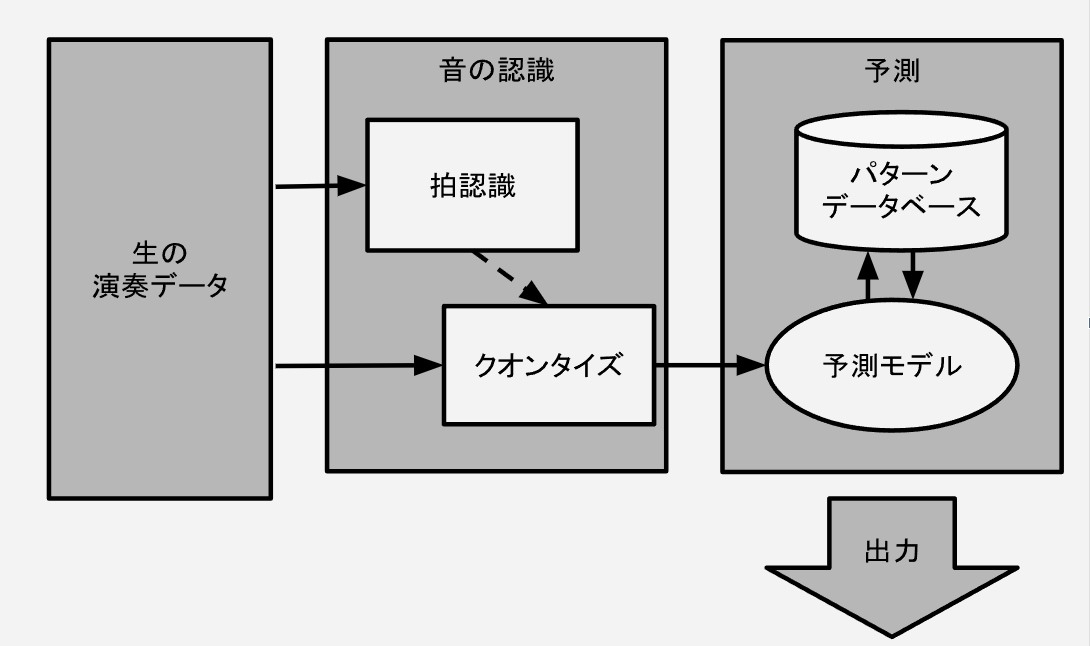
\includegraphics[width=0.8\linewidth]{src/pred.png}
  \caption{本システムの予測システム}
  \label{fig:tablenet}
\end{figure}

\section{位相修正}
受信部分において演奏相手の演奏予測を受け取った際,遅延を考慮して位相をずらして再生する必要がある.

\subsection{クロック同期}
OSCタイムタグはUNIX時間を基準にした絶対的な時間で送られるため,各クライアントのわずかな時計のずれで再生時間が変わってしまう.
そのため時計のずれを考慮したタイムタグの修正が必要である.
本システムでは簡易的であり,十分な精度が得られるという理由でCristianのアルゴリズム\cite{cristian}を採用している.

% TODO: 本システムで用いるクロック同期の開設計算式

%%% Local Variables:
%%% mode: japanese-latex
%%% TeX-master: "../bthesis"
%%% End:
